
\chapter[Introdução]{Introdução}

“Os requisitos de software expressam as necessidades e restrições impostas a um
produto que contribui para a solução de alguns problemas do mundo real” \cite{swebok2004}.

Partindo dessa afirmação, podemos entender que o processo de coleta de requisitos
é uma etapa crucial para a elaboração de um software, visto que nesta etapa são
levantados pontos para se entender as necessidades e o contexto onde tal software será inserido.

Este relatório tem por finalidade descrever e especificar todos os mecanismos e
etapas utilizados para levantar, especificar, gerenciar e analisar requisitos de um software.

\section{Visão Geral do Relatório}

Este relatório encontra-se organizado de acordo com os seguintes tópicos:

\begin{itemize}
		\item \textbf{Contexto do Cliente:} Conhecer a empresa e entender o problema a ser resolvido.
		\item \textbf{Abordagem de ER e Justificativa:} Explicar a abordagem escolhida, bem como as razões que
		conduziram sua escolha.
		\item \textbf{Processo de Engenharia de Requisitos:} Descrição do processo de levantamento e documentação
		dos requisitos.
		\item \textbf{Técnicas de Elicitação de Requisitos:} Descrição das técnicas que serão aplicadas para
		a elicitação de requisitos na segunda etapa do trabalho.
		\item \textbf{Gerenciamento de Requisitos:} Descrição dos processos que serão utilizados para a gerência
		de requisitos, bem como a ferramenta escolhida para este fim.
		\item \textbf{Planejamento do Projeto:} Descrição do planejamento de atividades e ferramentas adotadas.
\end{itemize}


\section{Contexto do Cliente}
A FGRacing é uma empresa júnior de Engenharia Automotiva, da Universidade de Brasília,
que constrói veículos de Fórmula SAE. A equipe trabalha em um projeto em um período de um ano,
e durante esse período os integrantes concentram as atenções na execução do projeto, levantamento fundos,
obtenção de patrocínio e divulgação do trabalho.

A empresa é estruturada em setores, de forma que um membro pode trabalhar em mais de um setor.
Por este motivo a divisão de trabalho pode tornar-se confusa e gerar sobrecarga em membros da equipe,
especialmente os que participam de atividades multi-setor.

O setor de marketing é essencial para o desenvolvimento da empresa, tanto na divulgação de seus
trabalhos quanto na obtenção de patrocinadores. Os maiores esforços deste setor se concentram em redes sociais.
Atualmente eles dispõem de um site, uma página no Facebook e Instagram como veículos de comunicação com o público.

Devido a sobrecarga de trabalho citada anteriormente, a FGRacing tem enfrentado dificuldades em criar conteúdo,
popular suas redes sociais e divulgar seus trabalhos. Por consequência, a empresa enfrenta dificuldades na obtenção
de patrocínios. No momento o site se encontra fora do ar, o Instagram está abandonado e o Facebook atuando como único
veículo de divulgação, ainda que não seja frequentemente utilizado.

\chapter[Abordagem da ER]{Abordagem da ER}

É amplamente reconhecido entre pesquisadores e profissionais da indústria que os projetos de software são criticamente
vulneráveis quando as atividades relacionadas a requisitos são mal executadas \cite{swebok2004}.

Todo o processo de produção de um software começa na Engenharia de Requisitos, pois ela é quem trabalhará no entendimento,
documentação, validação e gerenciamento do problema descrito pelo usuário, bem como sua solução.

Dada a natureza volátil e mutável dos requisitos, o processo de ER deve se ajustar à essas características, fornecendo um
firme arcabouço para o desenvolvimento adequado da solução exigida.

Visando garantir a qualidade da elaboração de softwares várias metodologias foram desenvolvidas ao longo dos anos, de acordo
com o contexto envolvido. Dentre as mais comuns podemos citar abordagens em cascata, iterativas, incrementais ou as modernas
abordagens ágeis. Para este projeto adotaremos a abordagem ágil, mais especificamente a metodologia SAFe, sintetizada a seguir.

\section{Scaled Agile Framework (SAFe)}
 SAFe é um framework que propõe boas práticas de desenvolvimento ágil, tendo uma estrutura baseada em práticas e padrões
 propostos e consolidados em outros frameworks, como: Lean, XP (eXtreme Programming), Scrum e Kanban \cite{dasilva2016}.

Este framework suporta o desenvolvimento em pequenas escalas (menos de 100 pessoas), mas tem o grande foco no desenvolvimento
empresarial com grandes e complexas produções de software.

Derivados dos lean e ágil, o SAFe apresenta os seguintes princípios:
\begin{itemize}
 	\item Adotar uma visão econômica
 	\item Aplicar pensamento sistêmico
 	\item Assumir variabilidade
 	\item Construir gradualmente com ciclos de aprendizagem rápidos e integrados
	\item Marcos básicos na avaliação objetiva dos sistemas de trabalho
	\item Visualizar e limitar WIP, reduzir tamanhos de lote e gerenciar comprimentos de fila
	\item Aplicar cadência, sincronizando com o planejamento entre domínios
 	\item Desbloquear a motivação intrínseca dos trabalhadores do conhecimento
 	\item Descentralizar a tomada de decisão
\end{itemize}

 O SAFe apresenta diversos benefícios, como aceleração do time-to-market, aumento da produtividade e da qualidade, e
 redução de riscos e custos do projeto \cite{turetken2016}.

 \begin{figure}[h]
 	\centering
 	\includegraphics[keepaspectratio=true,scale=0.2]{figuras/safe.eps}
 	\caption{SAFe}
 	\label{fig01}
 \end{figure}

\section{Justificativa da Abordagem}
\subsection{Panorama Ágil}
"Essencialmente, todos os modelos estão errados, mas alguns são úteis" \cite{box2005}.

A Engenharia de Software é uma área relativamente recente. Prova disto é que o termo software foi cunhado apenas em 1958,
por John Turkey \cite{swebok2004}. Durante toda sua existência, esta ciência tem se adaptado às tendências e mudanças
tecnológicas do mundo. Os métodos mais tradicionais como o cascata mostraram-se inadequados para a solução de todos os tipos
 de problemas, dada sua ineficiência na flexibilidade e revisão do projeto.

Com um mundo de tecnologias em constante mudança, os requisitos de software também seguem essa lógica. Os clientes podem
tomar decisões diferentes ao longo do projeto, motivados por novas tecnologias do mercado. Para atender à essa demanda,
as metodologias ágeis foram criadas, como uma resposta aos métodos tradicionais.

Seguem-se as razões pelas quais o grupo adotou a abordagem ágil para desenvolver o projeto.

\subsection{Cliente}
“Eu acredito profundamente na colaboração do usuário, e sem ela nada irá bem” \cite{glass2001}.

Partindo deste princípio, a abordagem ágil classificou-se como adequada ao projeto, visto que o cliente em questão (FGRacing)
 apresentou grande disponibilidade para reuniões. Ademais, o contato é facilitado pelo fato da sede da empresa ser localizada
  no Campus Gama da Universidade de Brasília, o mesmo local em que encontram-se os Analistas de Requisitos.

\subsection{Incertezas no Projeto}
Outro fator determinante foi a incerteza da empresa quanto ao produto final que deseja obter. Há diversas dúvidas sobre
como os problemas de marketing, criação de conteúdo e patrocínios serão resolvidos. Estas incógnitas podem ter influências
em diversas partes do software, desde o \textit{front-end} à sua arquitetura.

Glass acredita que “as mudanças nos requisitos são uma das causas mais comuns de falha de um projeto de software”,
e ainda que “clientes e usuários nem sempre sabem o que querem no início de um projeto de software, e devemos estar abertos
a mudanças durante a execução do projeto” \cite{glass2001}.

Para mitigar este risco, uma abordagem ágil é útil, em razão de suas características adaptativas.

\subsection{Documentação}
A empresa não demonstrou interesse específico em qualquer parte da documentação de software, o que não justificaria
uma abordagem mais tradicional como o RUP. A documentação será restritivamente funcional, ou seja, apenas o mínimo
necessário para o bom desenvolvimento do projeto.

\chapter[Processo de Engenharia de Requisitos]{Processo de Engenharia de Requisitos}
O SAFe é uma mescla entre XP, Scrum e Lean, tomando um conjunto de técnicas ágeis presentes nessas
três metodologias. O SAFe permite uma melhor interação entre os desenvolvedores, tendo uma abordagem bem documentada e
comprovada empiricamente. Esse framework possui uma comunicação eficiente entre os níveis estratégico, tático e operacional,
havendo um conjunto específico de práticas para cada um desses níveis organizacionais. O processo foi feito com a ferramenta
\textit{heflo} e é descrito da seguinte forma:

\begin{figure}[h]
	\centering
	\includegraphics[keepaspectratio=true,scale=0.35]{figuras/processo.eps}
	\caption{Processo de Engenharia de Requisitos}
	\label{fig03}
\end{figure}

\section{Subprocessos}
\begin{figure}[h]
	\centering
	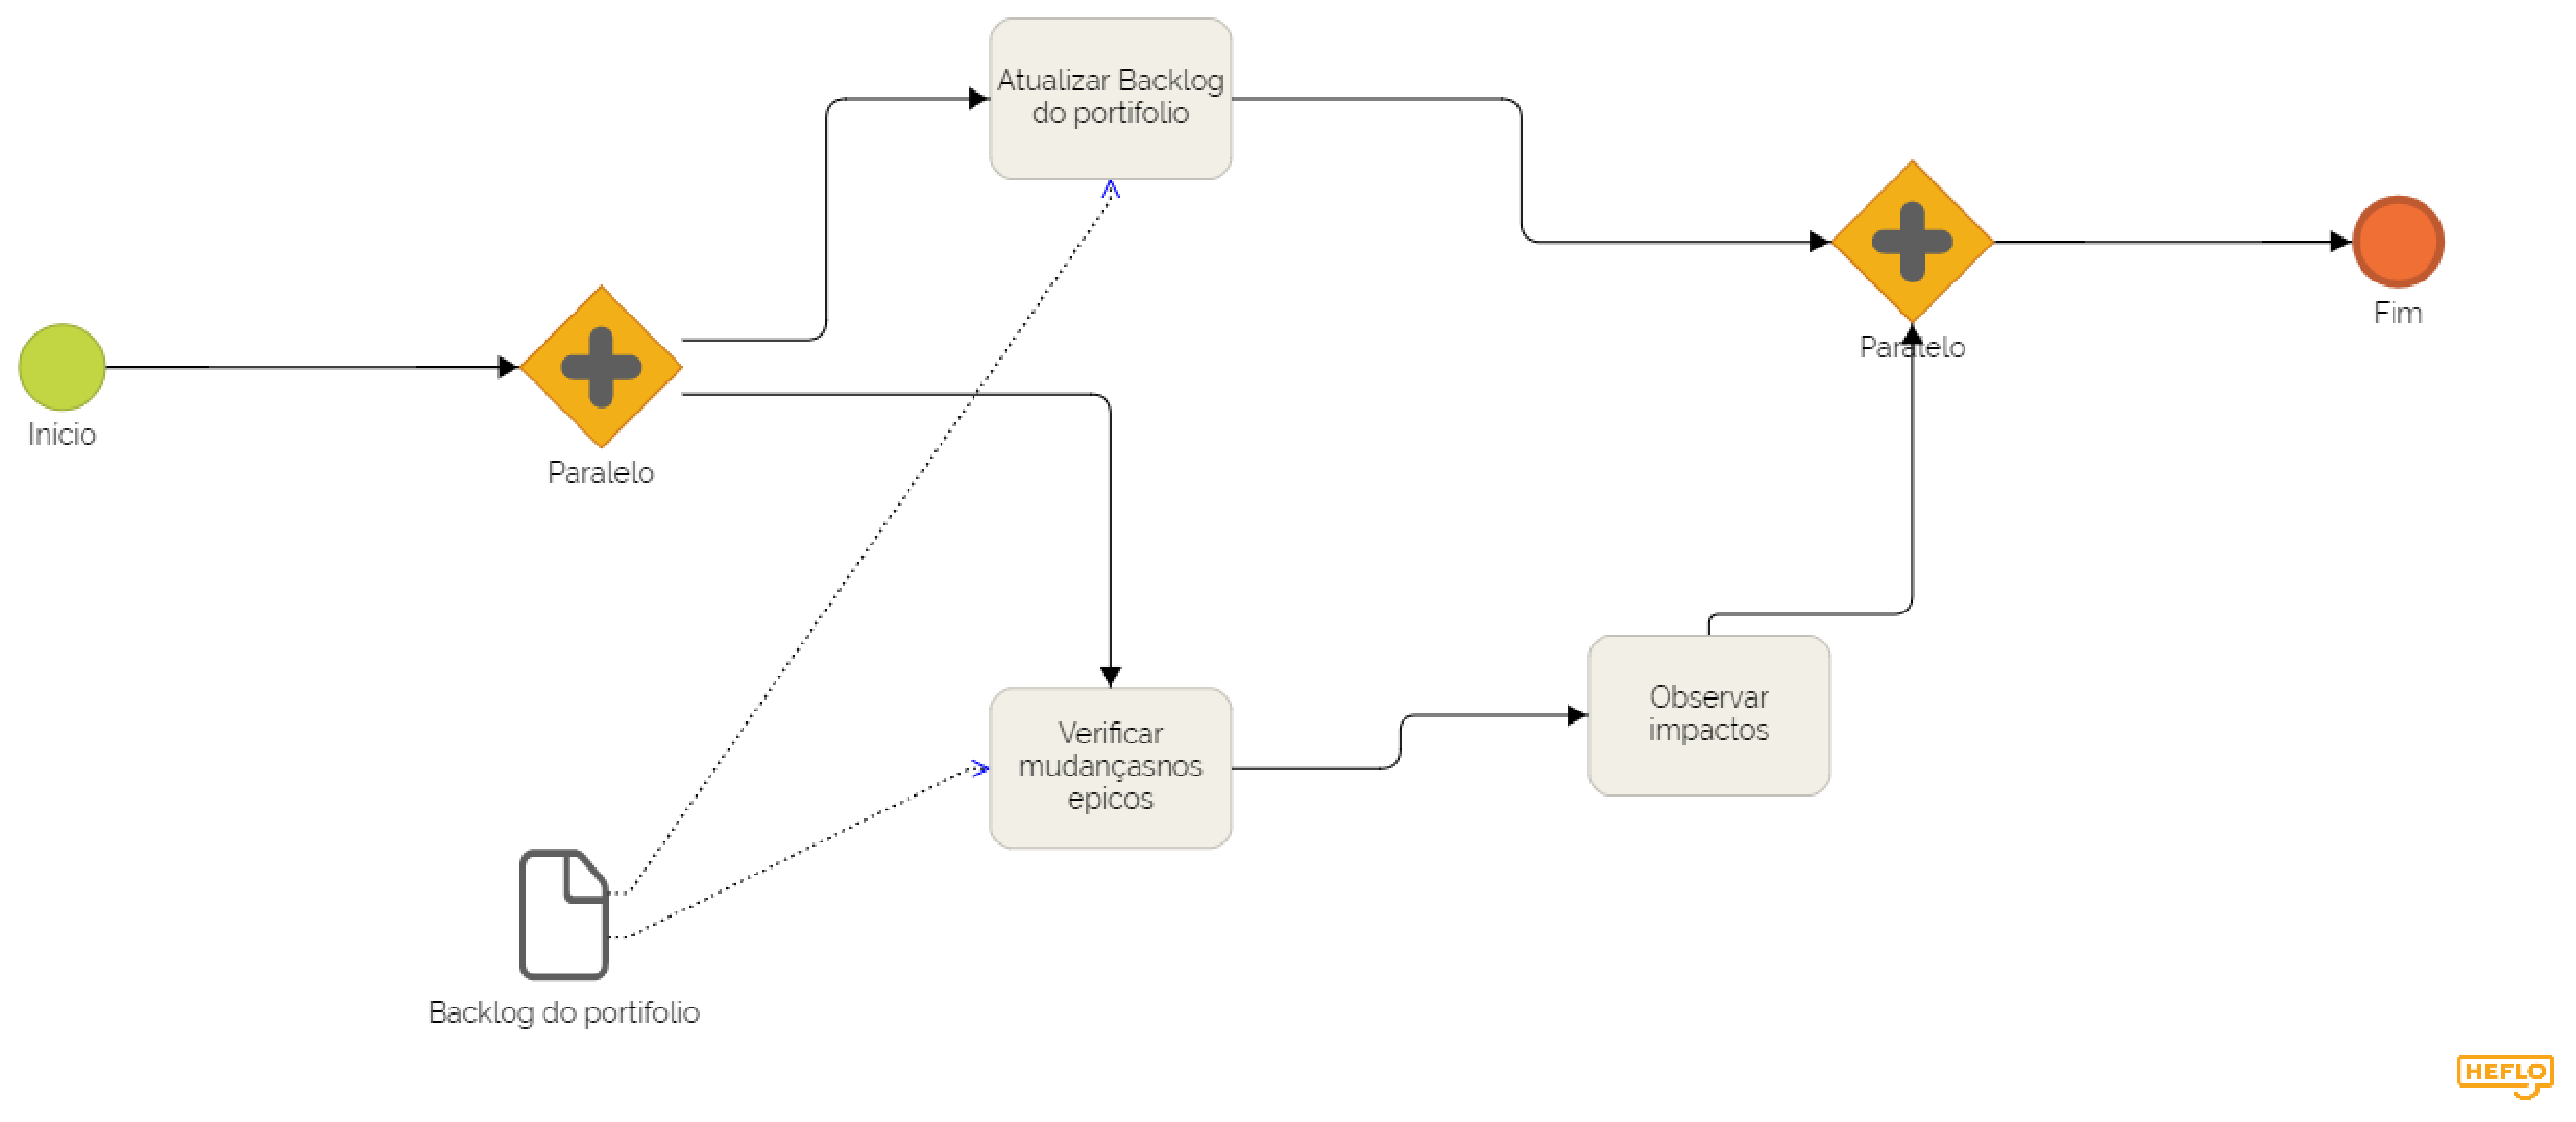
\includegraphics[keepaspectratio=true,scale=0.4]{figuras/subprocessoportfolio.eps}
	\caption{Gerência de Épicos}
	\label{fig04}
\end{figure}

\begin{figure}[h]
	\centering
	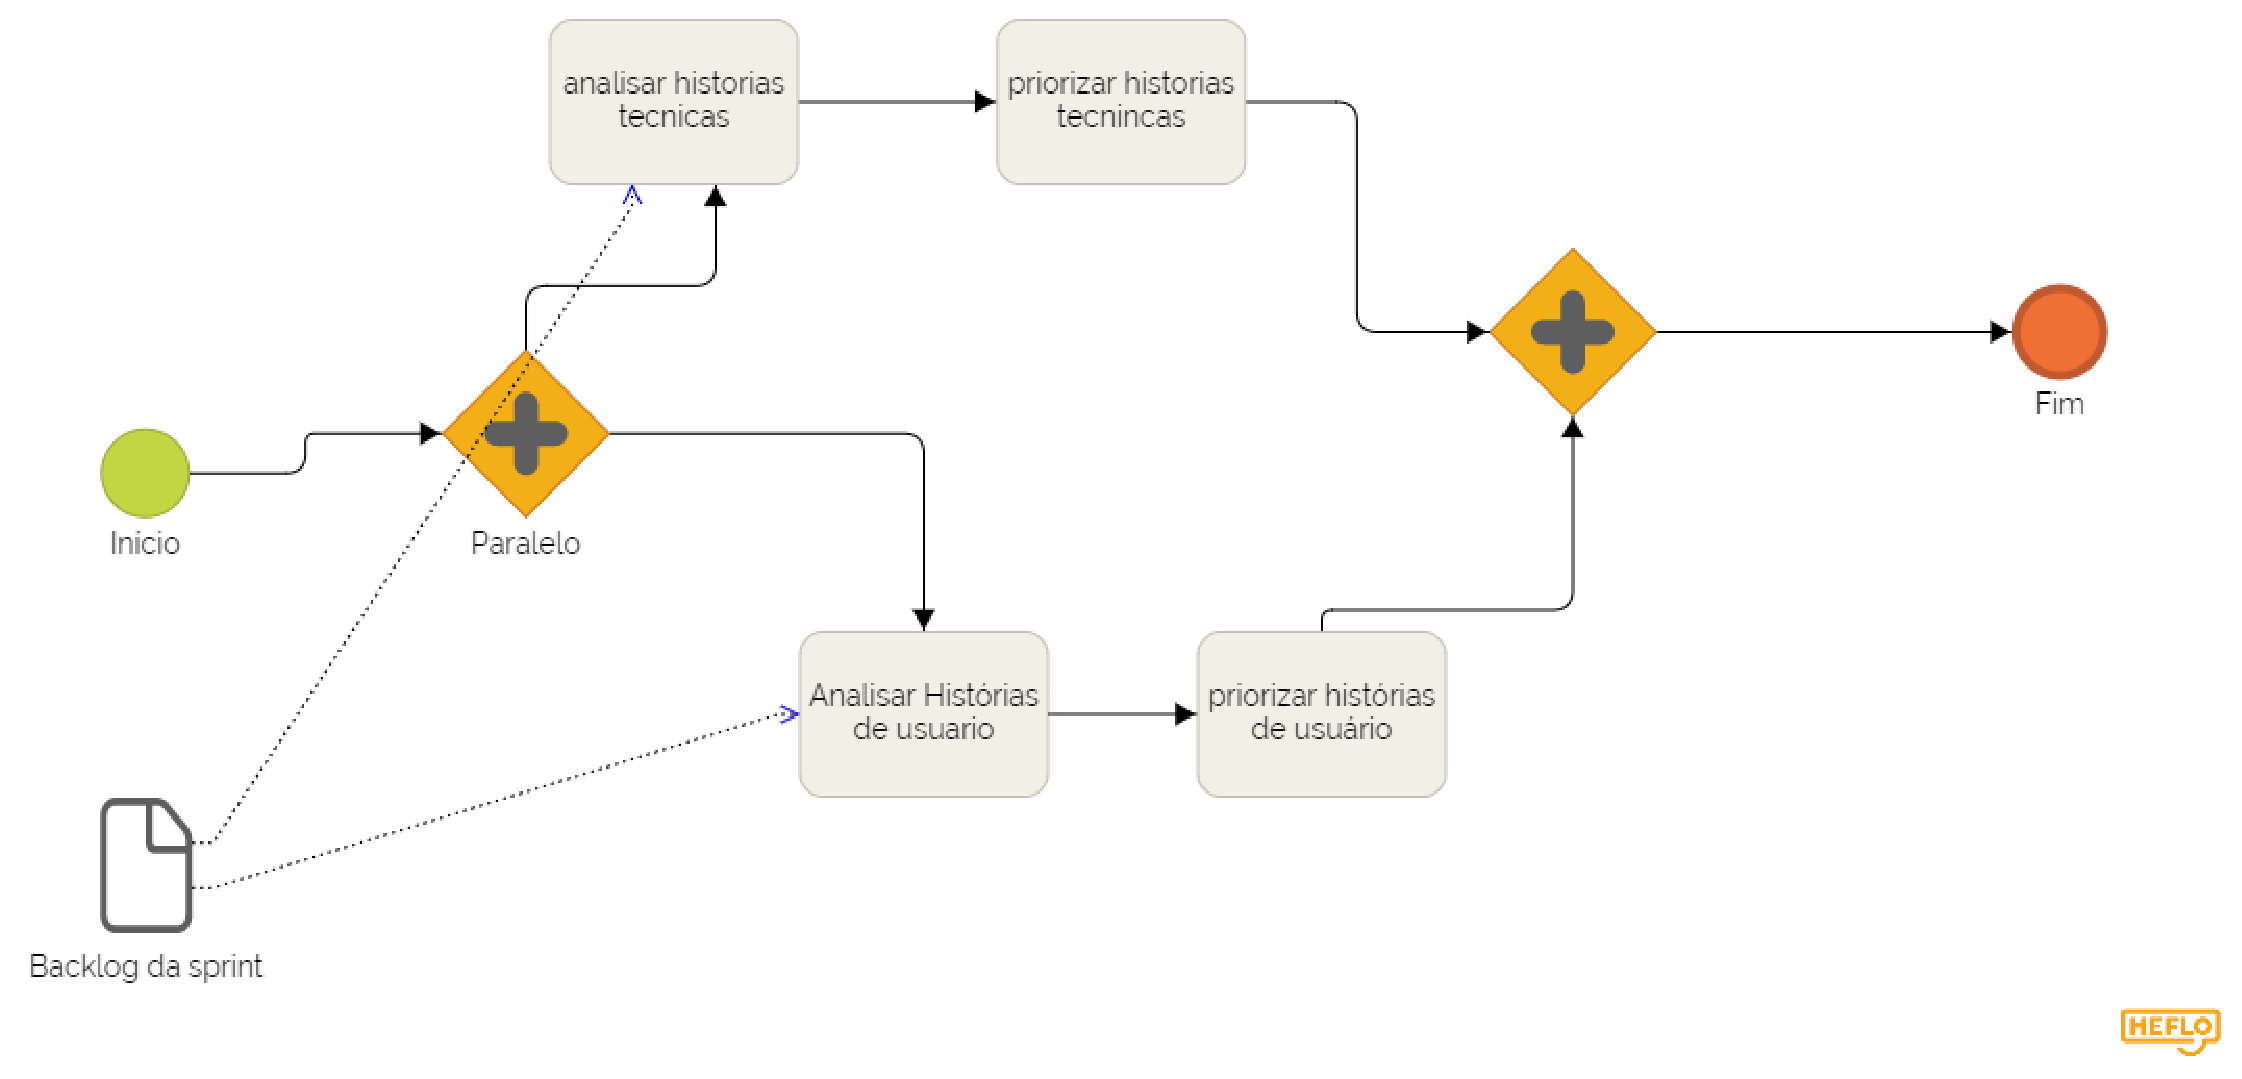
\includegraphics[keepaspectratio=true,scale=0.4]{figuras/gerencia.eps}
	\caption{Desenvolvimento da Sprint}
	\label{fig05}
\end{figure}

\section{Nível de Portfólio}
Esse nível tem por finalidade analisar e compreender o contexto do cliente, compreender o problema inicial,
observar características as quais levarão à criação de épicos. Os resultados obtidos serão efetivados mediante
as seguintes atividades:

\begin{itemize}
	\item Analisar o contexto da FGR
	\item Levantar épicos
	\item Identificar e detalhar épicos
	\item Efetivar épico
	\item Priorizar Épico
	\item Gerenciar épicos
\end{itemize}


A especificação das atividades pode ser observada segundo os diagramas a seguir que irão representar as entradas
e as saídas de cada uma delas:


\begin{table}[h]
	\centering
	\caption{Atividade 1}
	\label{my-label}
	\begin{tabular}{|l|l|}
	\hline
	\textbf{ID}       & 01                                                                    \\ \hline
	\textbf{Nome}     & Analisar o contexto da FGR                                            \\ \hline
	\textbf{Objetivo} & Realizar uma entrevista com o cliente a fim de compreender o problema \\ \hline
	\textbf{Entrada}  & Processo do projeto da FGR                                            \\ \hline
	\textbf{Saída}    & Tema de investimento                                                  \\ \hline
	\end{tabular}
\end{table}

\begin{table}[h]
	\centering
	\caption{Atividade 2}
	\label{my-label}
	\begin{tabular}{|l|l|}
		\hline
		\textbf{ID}       & 02                                                                        \\ \hline
		\textbf{Nome}     & Levantar Épicos                                                           \\ \hline
		\textbf{Objetivo} & Levantar conjunto de épicos analisados do tema de investimento da empresa \\ \hline
		\textbf{Entrada}  & Tema de investimento                                                      \\ \hline
		\textbf{Saída}    & Lista de Épicos do projeto                                                \\ \hline
	\end{tabular}
\end{table}

\begin{table}[h]
	\centering
	\caption{Atividade 3}
	\label{my-label}
	\begin{tabular}{|l|l|}
		\hline
		ID       & 03                                                  \\ \hline
		Nome     & Identificar e detalhar épicos                       \\ \hline
		Objetivo & Especificar e refinar os épicos previamente obtidos \\ \hline
		Entrada  & Lista de Épicos do projeto                          \\ \hline
		Saída    & Backlog do projeto                                  \\ \hline
	\end{tabular}
\end{table}

\begin{table}[h]
	\centering
	\caption{Atividade 4}
	\label{my-label}
	\begin{tabular}{|l|l|}
		\hline
		ID       & 04                               \\ \hline
		Nome     & Efetivar Épicos                  \\ \hline
		Objetivo & Efetivar os épicos identificados \\ \hline
		Entrada  & Épicos identificados             \\ \hline
		Saída    & Épicos refinados                 \\ \hline
	\end{tabular}
\end{table}

\begin{table}[h]
	\centering
	\caption{Atividade 5}
	\label{my-label}
	\begin{tabular}{|l|l|}
		\hline
		ID       & 05                                                                    \\ \hline
		Nome     & Priorizar Épicos                                                      \\ \hline
		Objetivo & Identificar os épicos mais relevantes para o funcionamento do sistema \\ \hline
		Entrada  & Lista de Épicos do projeto                                            \\ \hline
		Saída    & Backlog do projeto                                                    \\ \hline
	\end{tabular}
\end{table}

\begin{table}[h]
	\centering
	\caption{Atividade 6}
	\label{my-label}
	\begin{tabular}{|l|l|}
		\hline
		ID       & 06                                                                         \\ \hline
		Nome     & Gerência de Épicos                                                         \\ \hline
		Objetivo & Gerenciar ações e mudanças necessárias nos épicos brevemente identificados \\ \hline
		Entrada  & Lista de Épicos do projeto                                                 \\ \hline
		Saída    & Lista de Épicos do projeto                                                 \\ \hline
	\end{tabular}
\end{table}

\section{Nível de Programa}
No nível de programa as atividades se concentram em estabelecer diretrizes, caminhos e estratégias para a solução,
a partir dos levantamentos do contexto e consequentemente os requisitos que atenderão a demanda criada. Os resultados
obtidos serão efetivados mediante as seguintes atividades:

\begin{itemize}
	\item Selecionar Épicos
	\item Separar épicos em features
	\item Identificar requisitos não funcionais
	\item Levantar histórias de usuário
	\item Planejar release
	\item Entregar funcionalidades da release
\end{itemize}

\begin{table}[h]
	\centering
	\caption{Atividade 7}
	\label{my-label}
	\begin{tabular}{|l|l|}
	\hline
	\textbf{ID}       & 07                                                                 \\ \hline
	\textbf{Nome}     & Selecionar Épicos                                                  \\ \hline
	\textbf{Objetivo} & Separar Épicos em features e identificar requisitos não-funcionais \\ \hline
	\textbf{Entrada}  & Backlog do Portfólio                                               \\ \hline
	\textbf{Saída}    & Backlog do Portfólio                                               \\ \hline
	\end{tabular}
\end{table}

\begin{table}[h]
	\centering
	\caption{Atividade 8}
	\label{my-label}
	\begin{tabular}{|l|l|}
	\hline
	\textbf{ID}       & 08                         \\ \hline
	\textbf{Nome}     & Separar Épicos em Features \\ \hline
	\textbf{Objetivo} & Quebrar Épicos em Features \\ \hline
	\textbf{Entrada}  & Backlog do Portfólio       \\ \hline
	\textbf{Saída}    & Backlog do Portfólio       \\ \hline
	\end{tabular}
\end{table}

\begin{table}[h]
	\centering
	\caption{Atividade 9}
	\label{my-label}
	\begin{tabular}{|l|l|}
	\hline
	\textbf{ID}       & 09                                                       \\ \hline
	\textbf{Nome}     & Identificar requisitos não funcionais                    \\ \hline
	\textbf{Objetivo} & A partir dos Épicos, obter os requisitos não funcionais  \\ \hline
	\textbf{Entrada}  & Backlog do Portfólio                                     \\ \hline
	\textbf{Saída}    & Backlog do Portfólio                                     \\ \hline
	\end{tabular}
\end{table}

\begin{table}[h]
	\centering
	\caption{Atividade 10}
	\label{my-label}
	\begin{tabular}{|l|l|}
	\hline
	\textbf{ID}       & 10                            \\ \hline
	\textbf{Nome}     & Levantar histórias de usuário \\ \hline
	\textbf{Objetivo} & Levantar histórias de usuário \\ \hline
	\textbf{Entrada}  & Backlog do Portfólio          \\ \hline
	\textbf{Saída}    & Backlog do Time               \\ \hline
\end{tabular}
\end{table}

\begin{table}[!h]
	\centering
	\caption{Atividade 11}
	\label{my-label}
	\begin{tabular}{|l|l|}
	\hline
	\textbf{ID}       & 11                                                                                                                                      \\ \hline
	\textbf{Nome}     & Planejar Release                                                                                                                        \\ \hline
	\textbf{Objetivo} &\parbox[t]{7cm}{Planejar o que será feito e entregue até a release, estimar a quantidade de releases, datas de início e fim e as features implementadas} \\ \hline
	\textbf{Entrada}  & Backlog do Portfólio, Backlog do Time                                                                                                   \\ \hline
	\textbf{Saída}    & Roadmap                                                                                                                                 \\ \hline
	\end{tabular}
\end{table}

\begin{table}[!h]
	\centering
	\caption{Atividade 12}
	\label{my-label}
	\begin{tabular}{|l|l|}
	\hline
	\textbf{ID}       & 12                                    \\ \hline
	\textbf{Nome}     & Entregar Funcionalidades da Realease  \\ \hline
	\textbf{Objetivo} & Apresentar o que foi feito na release \\ \hline
	\textbf{Entrada}  & Backlog do Portfólio, Backlog do Time \\ \hline
	\textbf{Saída}    & Roadmap                               \\ \hline
	\end{tabular}
\end{table}


\section{Nível de Time}
No nível de time, os esforço de trabalho se concentram no desenvolvimento da solução. O principal objetivo é o planejamento
e a implementação das histórias de usuário, atendendo o contexto e as necessidades anteriormente já identificadas.

\begin{itemize}
	\item Priorizar e detalhar historia de usuários
	\item Planejar sprint
	\item Desenvolver sprint
	\item Retrospectiva da Sprint
\end{itemize}

\begin{table}[!h]
	\centering
	\caption{Atividade 13}
	\label{my-label}
	\begin{tabular}{|l|l|}
	\hline
	\textbf{ID}       & 13                                                                    \\ \hline
	\textbf{Nome}     & Priorizar e detalhar histórias de usuário                             \\ \hline
	\textbf{Objetivo} & Dar ênfases à histórias de usuário de acordo com a demanda do cliente \\ \hline
	\textbf{Entrada}  & Roadmap, Backlog do Time                                              \\ \hline
	\textbf{Saída}    & Backlog do Time (refinado)                                            \\ \hline
	\end{tabular}
\end{table}

\begin{table}[!h]
	\centering
	\caption{Atividade 14}
	\label{my-label}
	\begin{tabular}{|l|l|}
	\hline
	\textbf{ID}       & 14                                                                                                               \\ \hline
	\textbf{Nome}     & Planejar Sprint                                                                                                  \\ \hline
	\textbf{Objetivo} &\parbox[t]{7cm}{Planejar o caminhar da sprint, a alocação de pares, as histórias a serem implementadas e pontuação das histórias} \\ \hline
	\textbf{Entrada}  & Backlog do Time (refinado)                                                                                       \\ \hline
	\textbf{Saída}    & Backlog do Time (refinado)                                                                                       \\ \hline
	\end{tabular}
\end{table}

\begin{table}[!h]
	\centering
	\caption{Atividade 15}
	\label{my-label}
	\begin{tabular}{|l|l|}
	\hline
	\textbf{ID}       & 15                                           \\ \hline
	\textbf{Nome}     & Desenvolver Sprint                           \\ \hline
	\textbf{Objetivo} & Executar atividades planejadas para a sprint \\ \hline
	\textbf{Entrada}  &                                              \\ \hline
	\textbf{Saída}    & Módulos de Software                          \\ \hline
	\end{tabular}
\end{table}

\begin{table}[!h]
	\centering
	\caption{Atividade 16}
	\label{my-label}
	\begin{tabular}{|l|l|}
	\hline
	\textbf{ID}       & 16                                                                                                                      \\ \hline
	\textbf{Nome}     & Retrospectiva da Sprint                                                                                                 \\ \hline
	\textbf{Objetivo} &\parbox[t]{7cm}{Revisão do que foi executado durante a Sprint: pontos positivos e negativos, pontos a melhorar para as próximas sprints} \\ \hline
	\textbf{Entrada}  & Roadmap, Backlog do Time                                                                                                \\ \hline
	\textbf{Saída}    & Backlog do Time (refinado)                                                                                              \\ \hline
	\end{tabular}
\end{table}


\section{Mapeamento: Atividades Adotadas e Modelo de Maturidade}
O MPS.BR, Melhoria do Processo de Software Brasileiro, é um programa da Softex, o programa tem como objetivo melhorar a
capacidade de desenvolvimento de software, serviços e as práticas de gestão na indústria de Tecnologia, Inovação e Comunicação,
 o MPS apresenta 7 níveis de maturação estabelecendo níveis de capacidade e melhorias de processos, onde esses níveis são
 descritos de A a G.

Cada nível de maturidade possui suas áreas de processos, onde são analisados os processos fundamentais (todos os processos
que envolvem a elaboração dos requisitos e implantação do sistema), processos organizacionais (processos pertinentes a
gerência e organização da estrutura organizacional) e os processos de apoio (qualidade, configuração, validação e treinamento).
A capacidade do processo é representada por um conjunto de atributos de processo descrito em termos de resultados esperados.
Ela expressa o grau de refinamento e institucionalização com que o processo é executado na organização. No MPS, à medida que
a organização evolui nos níveis de maturidade, um nível de capacidade de desempenhar um processo deve ser atingido pela
organização. \cite{guia2012}.

Tendo cada um das atividades acima descritas, podemos mapeá-los para atender os resultados esperados do MPS-BR referentes às
atividades de engenharia de requisitos.

Os procedimentos foram mapeados como são demonstrados a seguir:

\section{Atividades}
	\subsection{Nivel de Portfólio}
		\begin{itemize}
			\item P01 - Analisar o contexto da FGR
			\item P02 - Levantar épicos
			\item P03 - Analisar e detalhar épicos
			\item P04 - Efetivar épicos
			\item P05 - Priorizar Épico
			\item P06 - Gerenciar épicos
		\end{itemize}

	\subsection{Nivel de Programa}
		\begin{itemize}
			\item Q01 - Selecionar épicos
			\item Q02 - Separar épicos em features
			\item Q03 - Identificar requisitos não funcionais
			\item Q04 - Levantar histórias de usuário
			\item Q05 - Planejar release
			\item Q06 - Entregar funcionalidades da release
		\end{itemize}

	\subsection{Nivel de Time}
		\begin{itemize}
			\item T01 - Priorizar historia de usuários
			\item T02 - Planejar sprint
			\item T03 - Desenvolver sprint
			\item T04 - Retrospectiva da Sprint
		\end{itemize}

	\subsection{Resultados Esperados}
		\subsubsection{Nível G - MPS-BR}
		GRE01 - O entendimento dos requisitos é obtido junto aos fornecedores de requisitos:

	O objetivo deste resultado é garantir que os requisitos estejam claramente definidos a partir do entendimento
	dos requisitos realizado junto aos fornecedores de requisitos. \cite{guia2012}.

	GRE02 - Os requisitos são avaliados com base em critérios objetivos e um comprometimento da equipe técnica com estes
	requisitos é obtido:

	A avaliação e aprovação por parte do cliente após o entendimento dos requisitos por si só não é suficiente para que os
	requisitos sejam refinados e refletidos em modelos de análise e projeto para a codificação. A avaliação dos requisitos
	deve envolver, além do cliente, também, a equipe técnica da organização, podendo ser realizada de diversas formas
	\cite{guia2012}.

	GRE03 - A rastreabilidade bidirecional entre os requisitos e os produtos de trabalho é estabelecida e mantida:

	Este resultado indica a necessidade de se estabelecer um mecanismo que permita rastrear a dependência entre os requisitos
	e os produtos de trabalho. Ter definida a rastreabilidade facilita a avaliação do impacto das mudanças de requisitos que
	possam ocorrer \cite{guia2012}.

	GRE04 - Revisões em planos e produtos de trabalho do projeto são realizadas visando a identificar e corrigir inconsistências
	em relação aos requisitos:

	A consistência entre os requisitos e os produtos de trabalho do projeto deve ser avaliada e os problemas identificados devem
	ser corrigidos. Este resultado sugere, portanto, a realização de revisões ou de algum mecanismo equivalente para identificar
	inconsistências entre os requisitos e os demais elementos do projeto como, por exemplo, planos, atividades e produtos de
	trabalho \cite{guia2012}.

	GRE05 - Mudanças nos requisitos são gerenciadas ao longo do projeto:

	Durante o projeto, os requisitos podem mudar por uma série de motivos. Desta forma, requisitos adicionais podem ser
	incorporados no projeto, requisitos podem ser retirados do projeto e/ou mudanças podem ser feitas nos requisitos já
	existentes \cite{guia2012}.

\subsubsection{Nível D - MPS-BR}
DRE01 - As necessidades, expectativas e restrições do cliente, tanto do produto quanto de suas interfaces, são identificadas:

O alcance deste resultado esperado envolve a utilização de métodos adequados para identificar necessidades, expectativas,
restrições e interfaces do cliente. Deve-se buscar o envolvimento de representantes do cliente e utilizar técnicas de
elicitação de requisitos para identificar de forma proativa requisitos adicionais não discutidos explicitamente pelos
clientes \cite{guia2012}

DRE02 - Um conjunto definido de requisitos do cliente é especificado e priorizado a partir das necessidades, expectativas
e restrições identificadas:

As necessidades, expectativas e restrições do cliente identificadas anteriormente são traduzidas em requisitos do
cliente \cite{guia2012}.

DRE03 - Um conjunto de requisitos funcionais e não-funcionais, do produto e dos componentes do produto que descrevem a solução
 do problema a ser resolvido, é definido e mantido a partir dos requisitos do cliente:

O alcance deste resultado esperado compreende a consolidação das necessidades, expectativas e restrições do cliente em um
conjunto de requisitos funcionais e não funcionais do produto e dos componentes do produto \cite{guia2012}.

DRE04 - Os requisitos funcionais e não-funcionais de cada componente do produto são refinados, elaborados e alocados

	Alcançar este resultado esperado significa elaborar os requisitos funcionais e não funcionais de cada componente do
	produto nos termos técnicos necessários para o desenvolvimento do produto e dos componentes do produto \cite{guia2012}.

DRE07 - Os requisitos são analisados, usando critérios definidos, para balancear as necessidades dos interessados com as
restrições existentes

Este resultado visa garantir que os requisitos, em seus diferentes níveis, sejam analisados de forma a balancear as
necessidades dos interessados com as restrições de projeto existentes \cite{guia2012}.

DRE08 - Os requisitos são validados

	Este resultado esperado visa garantir que os requisitos sejam validados utilizando-se técnicas adequadas, de forma a
	garantir que o produto terá o desempenho adequado quando instalado no seu ambiente alvo \cite{guia2012}.

\textit{As numerações seguem as numerações originais adotadas no Guia Geral MPS de Software, 2012.}

\section{Mapeamentos Resultados Esperados x Atividades}
	\begin{table}[!h]
	\centering
	\caption{Mapeamento dos Resultados Esperados x Atividades}
	\label{my-label}
	\begin{tabular}{|l|l|}
	\hline
	\textbf{Resultados Esperados} & \textbf{Atividades}                               \\ \hline
	\textbf{GRE01}                & P01, Q04                                          \\ \hline
	\textbf{GRE02}                & P02, P03, P04, P05, P06, Q02, Q04, T01            \\ \hline
	\textbf{GRE03}                & P03, P06 , Q01, Q02, Q04                          \\ \hline
	\textbf{GRE04}                & P01, P04, P06, Q05, T02, T03, T04                 \\ \hline
	\textbf{GRE05}                & P06                                               \\ \hline
	\textbf{DRE01}                & P01, P02, P03, P04 , P05, P06, Q01, Q03, Q04, T01 \\ \hline
	\textbf{DRE02}                & P03, P04, P05, P06, Q01, Q02, Q03, Q04, T01       \\ \hline
	\textbf{DRE03}                & P03, Q03                                          \\ \hline
	\textbf{DRE04}                & P03, P06, Q03                                     \\ \hline
	\textbf{DRE07}                & P03, P04, P05, P06                                \\ \hline
	\textbf{DRE08}                & P04                                               \\ \hline
	\end{tabular}
\end{table}

	\subsection{Resultados Esperados}

\textbf{GRE01 - P01, Q04:} O resultado esperado é obtido por meio da interação direta com o cliente.

\textbf{GRE02 - P02, P03, P04, P05, P06, Q02, Q04, T01:} O resultado esperado é atingido por meio do planejamento,
 do processo e organização da equipe técnica.

\textbf{GRE03 - P03, P06, Q01, Q02, Q04:} O resultado é alcançado por meio da organização dos requisitos visando manter a
consistência e a rastreabilidade.

\textbf{GRE04 - P01, P04, P06, Q05, T02, T03, T04:} O resultado esperado é alcançado por meio do constante acompanhamento
dos requisitos em todos os níveis visando a consistência e a efetividade dos requisitos.

\textbf{GRE05 - P06:} O resultado esperado é atingido por meio da adequação das atividades visando atender as necessidades
do cliente a todo momento.

\textbf{DRE01 - P01, P02, P03, P04 , P05, P06, Q01, Q03, Q04, T01:} Os resultados esperados são atingidos por meio dessas
atividades visando agradar o cliente no quesito usabilidade.

\textbf{DRE02 - P03, P04, P05, P06, Q01, Q02, Q03, Q04, T01:} O resultado é atingido por meio da priorização das atividades
ao longo do processo de desenvolvimento, com o objetivo de refinar a visão da equipe  de requisitos com relação aos
desejos do cliente.

\textbf{DRE03 - P03, Q03:} O resultado esperados é atingido por meio dessas atividades visando priorizar e detalhar os problemas
para adequar as necessidades do cliente.

\textbf{DRE04 - P03, P06, Q03:} O resultado esperado é atingido por meio da análise dos requisitos coletados com o objetivo de
definir quais são os requisitos funcionais e não funcionais.

\textbf{DR07 - P03, P04, P05, P06:} O resultado esperado é alcançado por meio de requisitos que se adequem corretamente as
necessidades e interesses do cliente.

\textbf{DRE08 - P04:} O resultado esperado é atingido por meio da conclusão e validação dos requisitos junto do cliente.

\chapter{Elicitação de Requisitos}
A Elicitação de Requisitos pode ser definida como o processo de compreensão dos requisitos dos \textit{stakeholders}
\cite{yousuf2015}, e o primeiro estágio para a construção do entendimento sobre o problema que o software deve resolver.
É um processo fundamentalmente humano onde são identificados os \textit{stakeholders} e estabelecidas as relações entre o cliente e o
 time de desenvolvimento \cite{swebok2004}.

	Para fazer um levantamento de requisitos que supra as necessidades do cliente de forma satisfatória, é necessário um total
	entendimento sobre diferentes áreas, como o domínio da aplicação, regras de negócio, restrições, e o problema em si
	\cite{paetsch2003}. Para isso, existem diversas técnicas para elicitação de requisitos. Algumas destas podem ser mais adequadas
	 a um determinado contexto que outras, por isso foram selecionadas cinco técnicas as quais foram julgadas adequadas ao
	  problema descrito por este relatório. São elas Brainstorming, Entrevistas, Questionários, Observação e Cenários.

\section{Entrevistas}
Este método tem como objetivo descobrir fatos e opiniões de stakeholders sobre o sistema em desenvolvimento \cite{paetsch2003}.
 É muito popular e considerado como uma técnica importante para obter e validar requisitos. A entrevista consiste em uma
 conversa face a face onde se discute com diferentes tipos de stakeholders, buscando entender os requisitos do sistema e seus
 objetivos para solucionar o problema.

Existem dois tipos de entrevista:

\begin{itemize}
	\item \textbf{Entrevista Fechada:} Onde o engenheiro de requisitos tem uma série de perguntas pré-definidas que serão feitas para o
entrevistado.

	\item \textbf{Entrevista Aberta:} Onde não existem perguntas pré-definidas. O engenheiro de requisitos e os stakeholders discutem abertamente
 sobre o que esperam do sistema.
\end{itemize}

Em alguns casos, em entrevistas fechadas, assuntos consideráveis podem surgir, levando a uma discussão aberta. Nestes casos,
alguns autores descrevem um tipo semiestruturado de entrevista, que mescla os atributos de reuniões abertas e fechadas
\cite{yousuf2015}.
Métodos ágeis afirmam que as entrevistas são uma maneira eficiente de se comunicar com o cliente, e resultam em um aumento de
 confiança entre os dois lados \cite{delucia2010}.

 \section{Observação}
Também conhecido como “Análise Social”, este método consiste em coletar requisitos observando usuários em seu ambiente sem
 interferir em seu trabalho. É utilizado geralmente para encontrar requisitos quando os stakeholders não conseguem expressar
  muito bem os requisitos esperados para o sistema \cite{gunda2008}.

Existem diferentes maneiras de aplicar esta técnica. O engenheiro de requisitos pode observar diretamente, estando presente
 durante a atividade do usuário, ou indiretamente, por meio de gravações de áudio e vídeo.

 \section{Brainstorming}
 Brainstorming é uma técnica de grupo utilizada para criar novas ideias para o projeto e/ou encontrar soluções para um problema
  específico, além de possibilitar o diagnóstico de problemas em pouco tempo. São conduzidos como uma conferência reunindo de
	seis a dez membros, onde cada membro tem o direito de explanar suas ideias em um certo período de tempo. Esta reunião possui
	 um mediador, que define a questão a ser discutida \cite{gunda2008}.

 Todas as ideias geradas são anotadas, e ao fim da fase criativa, são avaliadas por todos os membros. As ideias inapropriadas
  são excluídas e as mais apropriadas priorizadas.

\chapter{Gerenciamento de ER}
Para que ferramentas de requisitos trabalhem eficientemente “elas devem ser capaz de armazenar, priorizar, mudanças nas exigências de faixa
 e desenvolvimento, e proporcionar um nível de rastreabilidade de requisitos” \cite{delucia2010}.

\section{Técnicas de Rastreabilidade de Requisitos}
Rastreabilidade pode ser definida como sendo a técnica usada para promover relacionamento entre requisitos, arquiteturas e
implementação final do sistema \cite{edwards1991}. Ela auxilia na compreensão dos relacionamentos existentes entre requisitos
 do software ou entre artefatos de requisitos, arquitetura e implementação. Esses relacionamentos permitem aos projetistas
  mostrar que o projeto atende aos requisitos. A rastreabilidade também apóia a detecção precoce daqueles requisitos não
	atendidos pelo software (Palmer, 1997).

A Rastreabilidade de Requisitos também é definida como a capacidade de descrever e seguir o ciclo de vida de um requisito
em ambas as direções: na capacidade de rastrear um artefato em direção à sua implementação (\textit{forward traceability}); ou na
capacidade de rastrear um artefato à sua origem (\textit{backward traceability}); passando entre todas as especificações relatadas
(GOTEL, 1994).

Sobre os tipos de rastreabilidade, existem basicamente duas classificações gerais: horizontal e vertical e pré e
pós-rastreabilidade \cite{finkelstein1995}.



\begin{itemize}
	\item \textbf{Pré-rastreabilidade:} pode ser  definida como os documentos obtidos no processo de elicitação de requisitos mapeando as dependências com artefatos prévios.
	\item \textbf{Pós-rastreabilidade:} envolver as informações obtidas por atividades subsequentes de desenvolvimento.
\end{itemize}
\newpage
\begin{figure}[h]
	\centering
	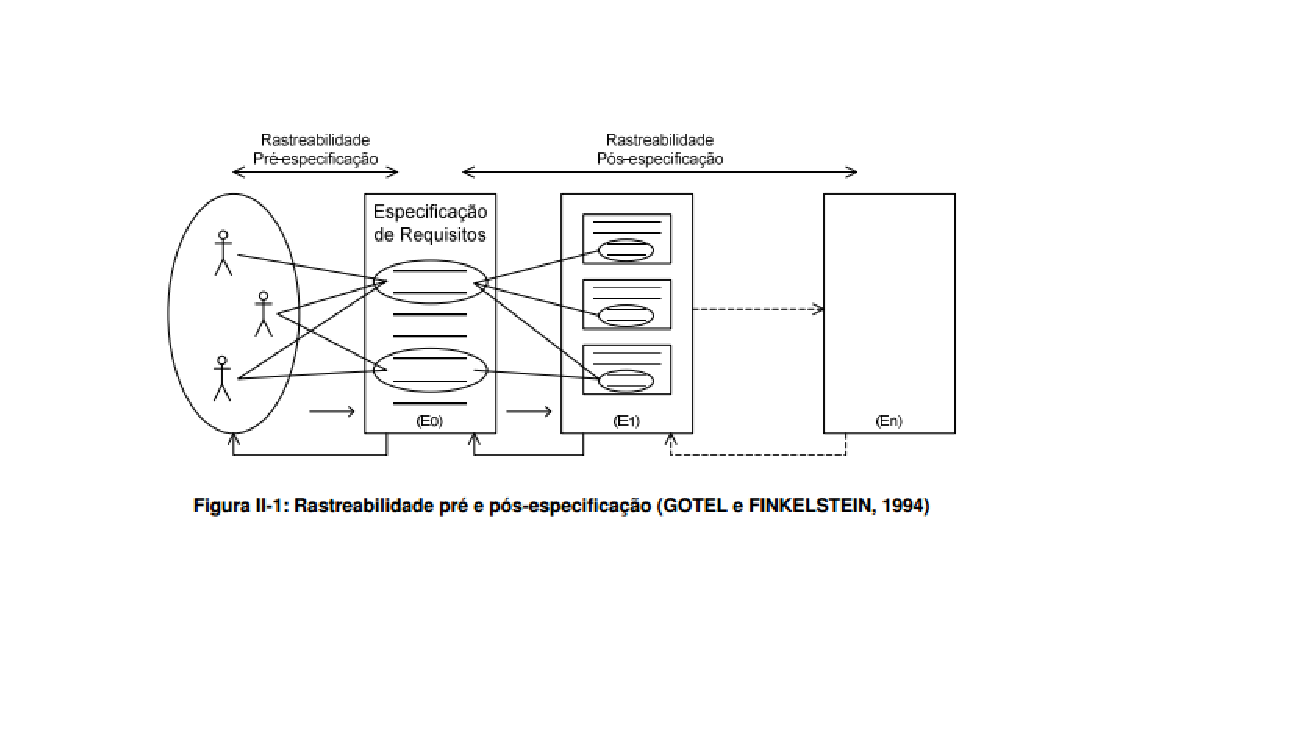
\includegraphics[keepaspectratio=true,scale=0.9]{figuras/rastreabilidade_ida_e_volta.eps}
	\caption{Pré-Rastreabilidade}
	\label{fig05}
\end{figure}

A rastreabilidade também pode ser categorizada como horizontal (inter-rastreabilidade) e vertical (extra rastreabilidade)
 \cite{sommerville1998}.

\begin{itemize}
	\item \textbf{Rastreabilidade horizontal:} é a rastreabilidade entre diferentes versões ou variações de requisitos, ou outros
	artefatos, em uma particular fase do ciclo de vida, ou seja, permite ver como os requisitos relacionam-se com os demais
	requisitos.
	\item \textbf{Rastreabilidade vertical:} é realizada entre requisitos e artefatos produzidos pelo processo de desenvolvimento
	 ao longo do ciclo de vida do projeto, ou seja, permite ver como os requisitos relacionam-se com os artefatos que são gerados
	  no decorrer do projeto \cite{genvigir2009}.
\end{itemize}
\newpage
\begin{figure}[h]
	\centering
	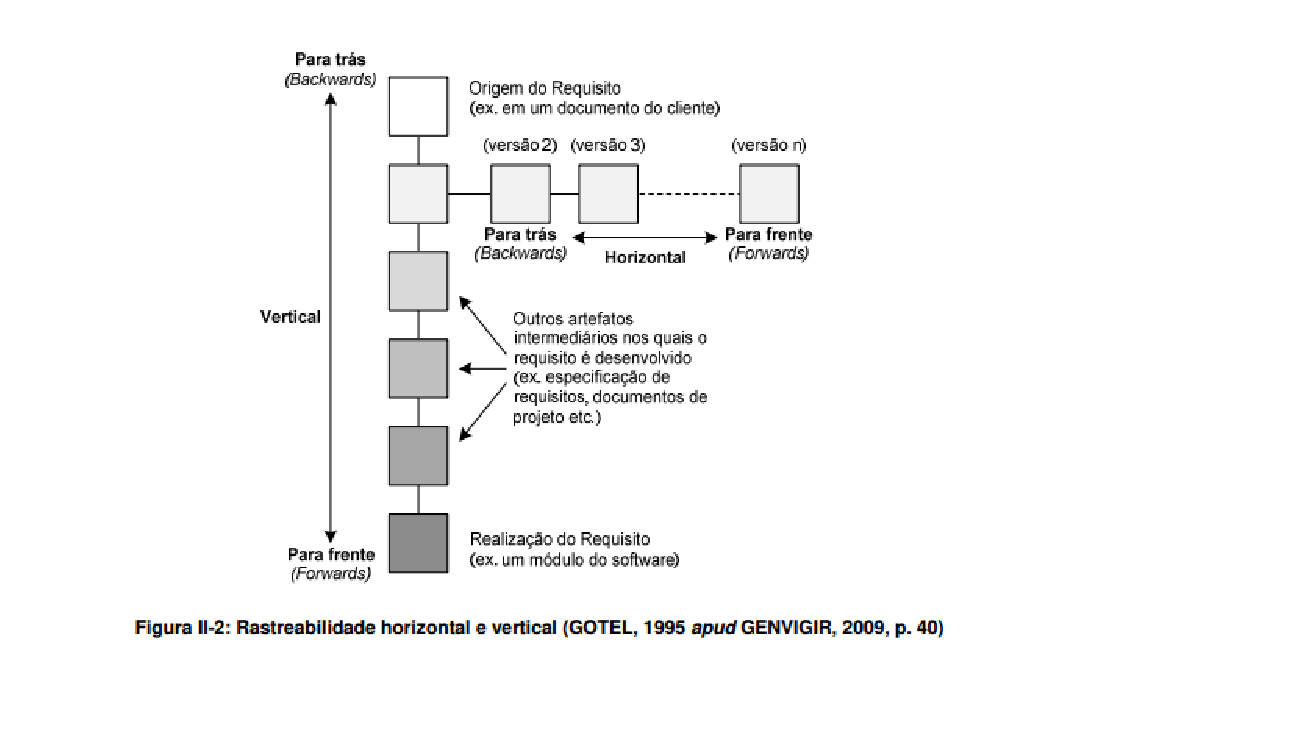
\includegraphics[keepaspectratio=true,scale=0.9]{figuras/Rastreabilidade_Horizontal_vertical.eps}
	\caption{Rastreabilidade}
	\label{fig06}
\end{figure}

Tendo como base os conceitos apresentados sobre as técnicas de rastreabilidade de requisitos, adotamos a rastreabilidade
 horizontal e vertical onde poderemos ter a rastreabilidade dos requisitos desde tema de investimento até as histórias de
  usuário como mostrados a seguir:

\begin{itemize}
	\item \textbf{TI\#} - Temas de investimento
	\item \textbf{EP\#} - Épicos
	\item \textbf{FT\#} - Features
	\item \textbf{H\#} - Histórias de Usuário
\end{itemize}

\textit{as “\#” representam índices numéricos}

\section{Atributos de Requisitos}
Requisitos não são determinados apenas pelas suas especificações e detalhes do que é extraído do cliente, mas também por
 um conjunto de informações a respeito deles, os quais permitem uma melhor interpretação e entendimento, essas informações
  são definidas como atributos de rastreabilidade de requisitos.

	Para a realização deste trabalho foram definidos os seguintes atributos:

	\begin{itemize}
		\item Origem
		\item Prioridades
		\item Status
		\item Grau de dificuldade
	\end{itemize}

\textbf{Origem:} Os requisitos possuirão identificadores seguidos de índices numéricos para serem únicos.

\begin{table}[!h]
	\centering
	\caption{Identificadores de Atributos de Requisitos}
	\label{my-label}
	\begin{tabular}{|l|l|}
	\hline
	\textbf{TI\#} & Temas de Investimetno \\ \hline
	\textbf{EP\#} & Épicos                \\ \hline
	\textbf{FT\#} & Features              \\ \hline
	\textbf{H\#}  & Histórias de Usuário  \\ \hline
	\end{tabular}
\end{table}

\textbf{Status:} o status irá indicar o grau de implementação do requisito no sistema, sendo divido em, em progresso, não iniciado,
 concluído

- Em progresso: indica que o requisito já está em processo de implementação

- Não iniciado: o requisito não não foi iniciada a sua implementação

- Concluído: o requisito previamente descrito já encontra-se implementado no sistema

\textbf{Prioridade:} indicará o grau de necessidade de implementação daquele requisito no sistema, a prioridade poderá ser alta, média e baixa.

- Alta: quando o requisito for avaliado pelo stakeholders como crucial, ou caso sem esse requisito o sistema não consegue funcionar.

- Média: quando o requisito tem relevância para os interessados, mas que sem a implementação dele o sistema consegue manter o funcionamento.

- Baixa: quando o requisito não compromete o funcionamento do requisito.

\textbf{Grau de dificuldade:} indica a dificuldade de implementação do requisito no sistema, também sendo divido em alta, média e baixa.

- Alta: requisito que necessita de grande esforço da equipe para a sua implementação.

- Médio: requisito que exige esforço moderado da equipe para a sua implementação.

- Baixo: requisito que exige pouco esforço para a sua implementação.

\chapter{Ferramenta de Gestão de Requisitos}
Para se ter uma maior visão e administração dos requisitos, é necessária uma  ferramenta que auxilie nessas atividades,
proporcionando uma melhor rastreabilidade, manutenção dos atributos dos requisitos, relacionamento entre os requisitos e
gestão de mudanças.

Em busca de uma ferramenta que atendesse essas demandas foi realizada uma pesquisa, com o intuito de comparar e selecionar a
 ferramenta de melhor uso para a equipe e melhor realização das tarefas. Foram comparadas 3 ferramentas: sendo elas TraceCloud,
  Taiga e Mingle

\section{Ferramentas}
	\subsection{TraceCloud}
	TraceCloud é uma solução em Gerência de Requisitos web, flexível ao qual pode tanto ser utilizada para metodologias ágeis
	quantos tradicionais, ela possui sistemas de rastreabilidade, validação, compartilhar requisitos, aprovações de trabalhos,
	 segurança com bloqueios e controle de alterações entre outros.

	 \begin{figure}[!h]
	 	\centering
	 	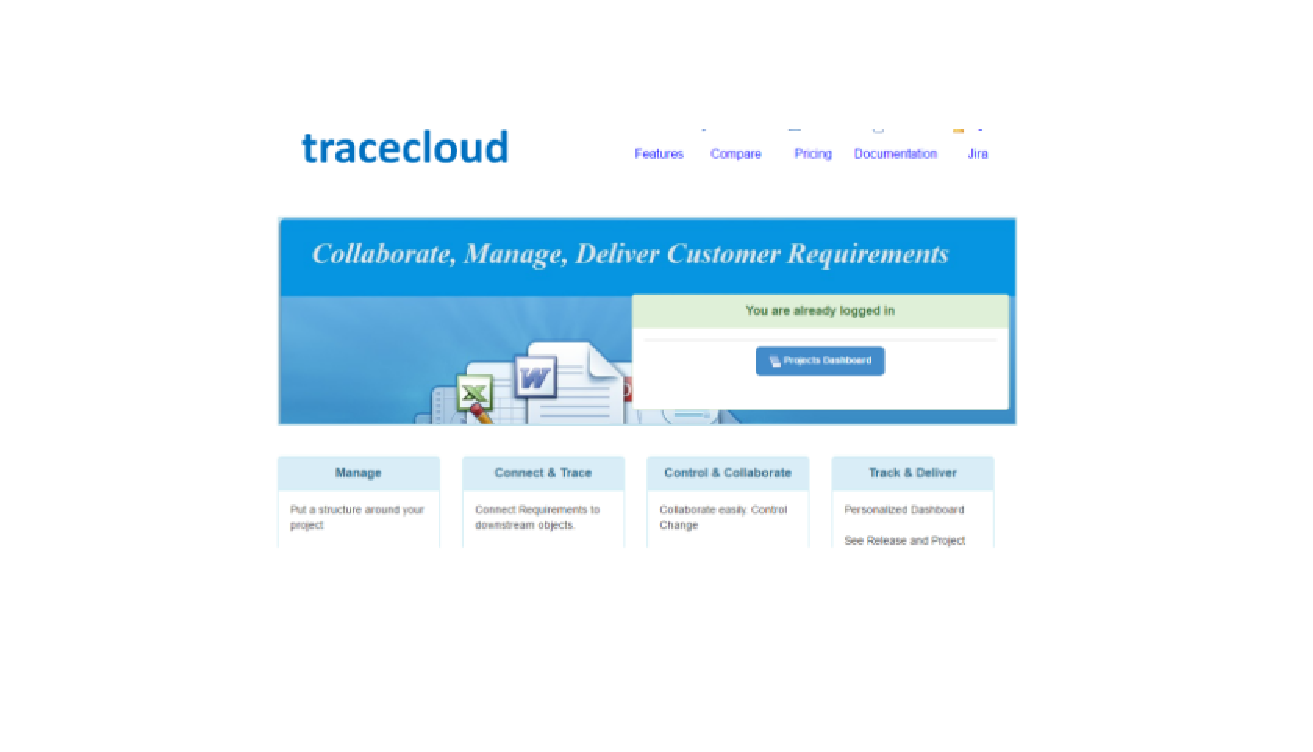
\includegraphics[keepaspectratio=true,scale=0.75]{figuras/tracecloud1.eps}
	 	\caption{Ferramenta TraceCloud}
	 	\label{fig07}
	 \end{figure}

	 \begin{figure}[!h]
	   \centering
	   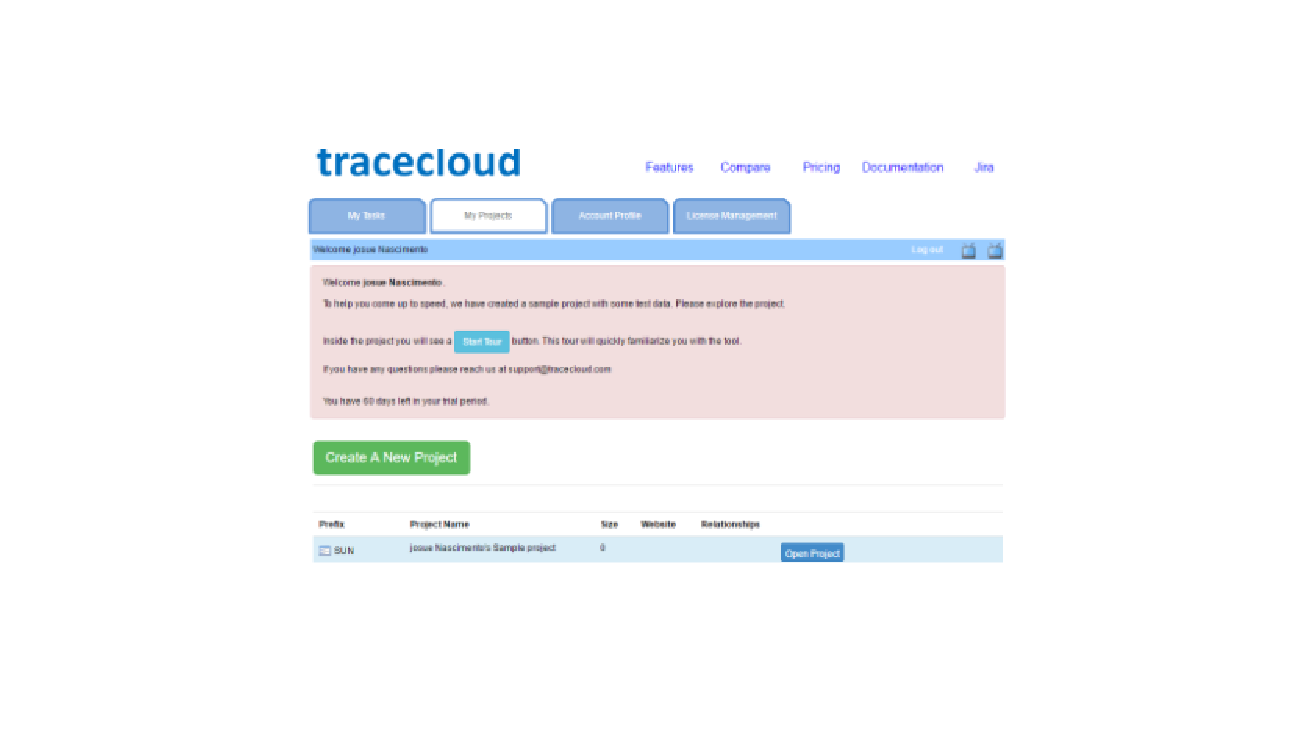
\includegraphics[keepaspectratio=true,scale=0.8]{figuras/tracecloud2.eps}
	   \caption{Ferramenta TraceCloud}
	   \label{fig08}
	 \end{figure}

	 \begin{figure}[!h]
	   \centering
	   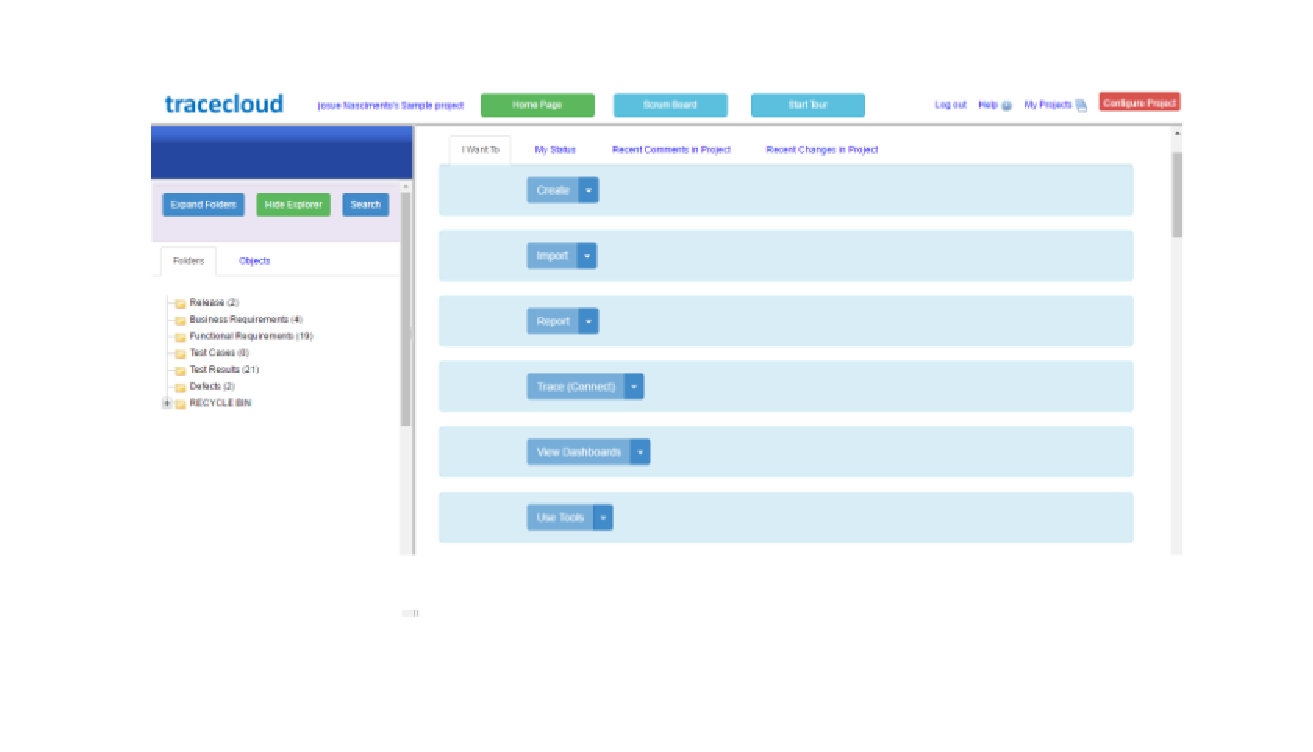
\includegraphics[keepaspectratio=true,scale=0.7]{figuras/tracecloud3.eps}
	   \caption{Ferramenta TraceCloud}
	   \label{fig09}
	 \end{figure}

	 \subsection{Taiga}
	 Ela fornece funções de backlogs, boards no estilo Kanban, gerenciadores de tarefas, sprints e muito mais. As integrações
	 com outras ferramentas são simples e se há qualquer dificuldade em sua utilização, pode-se recorrer à comunidade Taiga,
	 para projetos abertos, as funções são totalmente gratuitas, independentemente do tamanho do time. Enquanto times de até
	 4 pessoas trabalhando em 1 projeto privado também podem utilizar a solução gratuitamente.

	 \begin{figure}[!h]
	   \centering
	   \includegraphics[keepaspectratio=true,scale=0.45]{figuras/taiga1.eps}
	   \caption{Ferramenta Taiga}
	   \label{fig10}
	 \end{figure}

	 \begin{figure}[!h]
		 \centering
		 \includegraphics[keepaspectratio=true,scale=0.45]{figuras/taiga2.eps}
		 \caption{Ferramenta Taiga}
		 \label{fig11}
	 \end{figure}

	 \begin{figure}[!h]
		 \centering
		 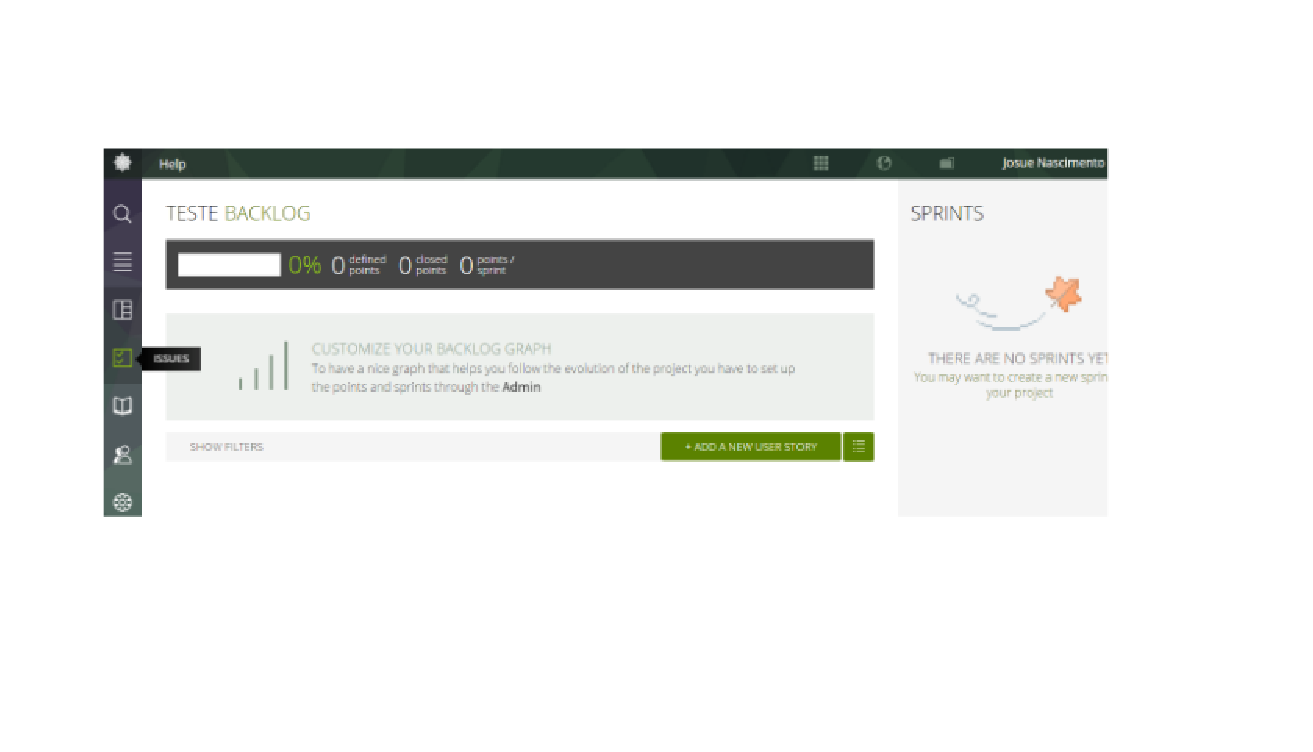
\includegraphics[keepaspectratio=true,scale=0.9]{figuras/taiga3.eps}
		 \caption{Ferramenta Taiga}
		 \label{fig12}
	 \end{figure}

 \subsection{Mingle}
	 Mingle é uma ferramenta simples e poderosa. Trata-se de uma ferramenta web feita com a gestão ágil de projetos e a
	 colaboração entre times em mente, fornecendo um ambiente de trabalho completo para toda a equipe. Dispõe de funcionalidades
	  como fóruns, quadro kanban, wiki e integração com código fonte.

	\begin{figure}[!h]
 		 \centering
 		 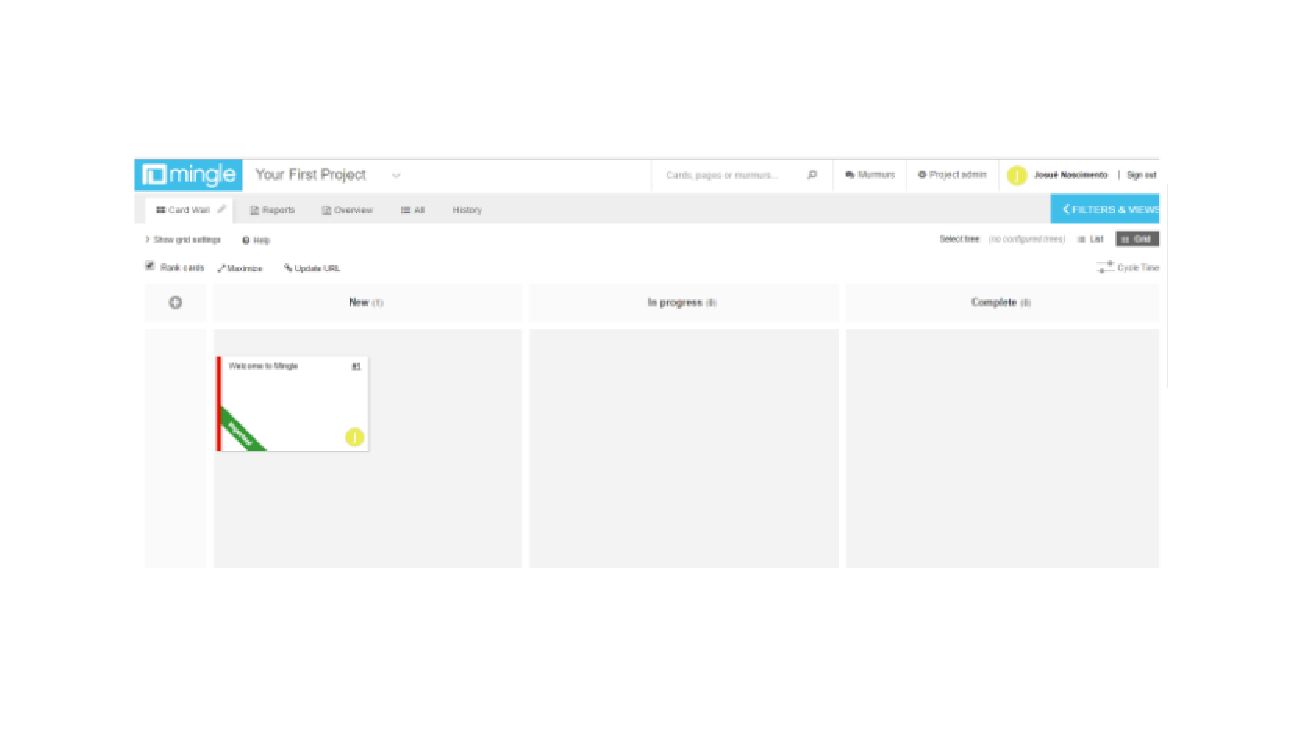
\includegraphics[keepaspectratio=true,scale=0.59]{figuras/mingle1.eps}
 		 \caption{Ferramenta Mingle}
 		 \label{fig13}
 	\end{figure}

	\begin{figure}[!h]
		 \centering
		 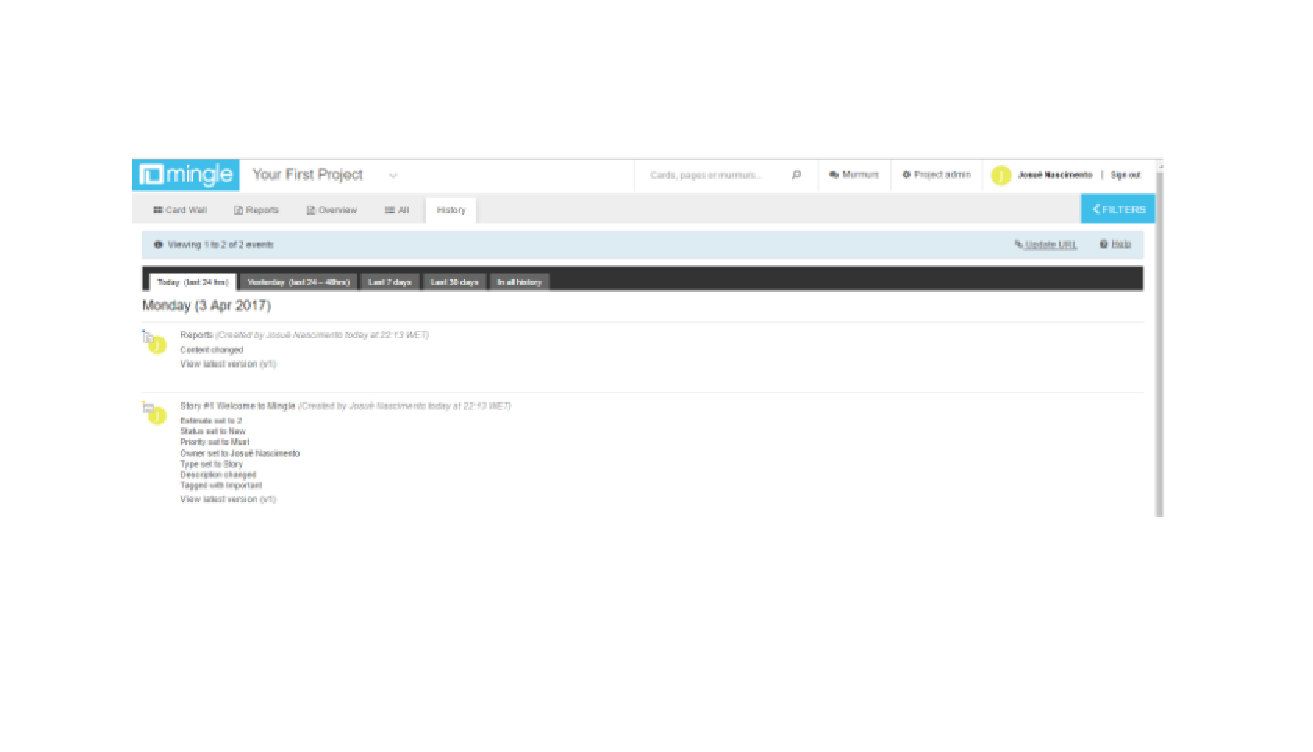
\includegraphics[keepaspectratio=true,scale=0.75]{figuras/mingle2.eps}
		 \caption{Ferramenta Mingle}
		 \label{fig14}
	\end{figure}

\section{Análise das Ferramentas}
 		\subsection{Critérios de Análises}
		Para a escolha da ferramenta a ser utilizada foi levado em conta os seguintes aspectos:

		\begin{itemize}
			\item Usabilidade
			\item Gestão de mudanças
			\item Rastreabilidade
			\item Flexibilidade
			\item Licensa
		\end{itemize}

\begin{table}[!h]
\centering
	\caption{Critérios de Análise de Ferramentas}
	\label{my-label}
	\begin{tabular}{|l|l|}
	\hline
	\textbf{Critério}          & \textbf{Descrição}                                                                   \\ \hline
	\textit{Usabilidade}       & Retrata o desempenho dos usuários em trabalhar com o software                        \\ \hline
	\textit{Ratreabilidade}    & Realizar a rastreabilidade entre os requisitos                                       \\ \hline
	\textit{Gestão de Mudança} &\parbox[t]{7cm}{O gerenciamentos de atividades em relação aos processos, de engenharia de requisitos} \\ \hline
	\textit{Flexibilidade}     & Permitir que vários usuários tenham acesso ao mesmo projeto                          \\ \hline
	\textit{Licensa}           & Se é gratuito ou não                                                                 \\ \hline
	\end{tabular}
\end{table}

Os critérios foram pontuados com base na seguinte tabela:

\begin{table}[!h]
	\centering
	\caption{Pontos Para Ferramentas}
	\label{my-label}
	\begin{tabular}{|l|l|}
	\hline
	\textbf{Análise} & \textbf{Pontos} \\ \hline
	\textit{Alta}    & 3               \\ \hline
	\textit{Média}   & 2               \\ \hline
	\textit{Baixa}   & 1               \\ \hline
	\end{tabular}
\end{table}

		\subsection{Escolha da Ferramenta}
		Segundo foi especificado, cada um dos membros da equipe testou todas ferramentas, onde durante o teste, foram pontuando cada
		 	um dos critérios, os resultados obtidos está descrito na tabela a seguir:


			\begin{figure}[!h]
			\centering
			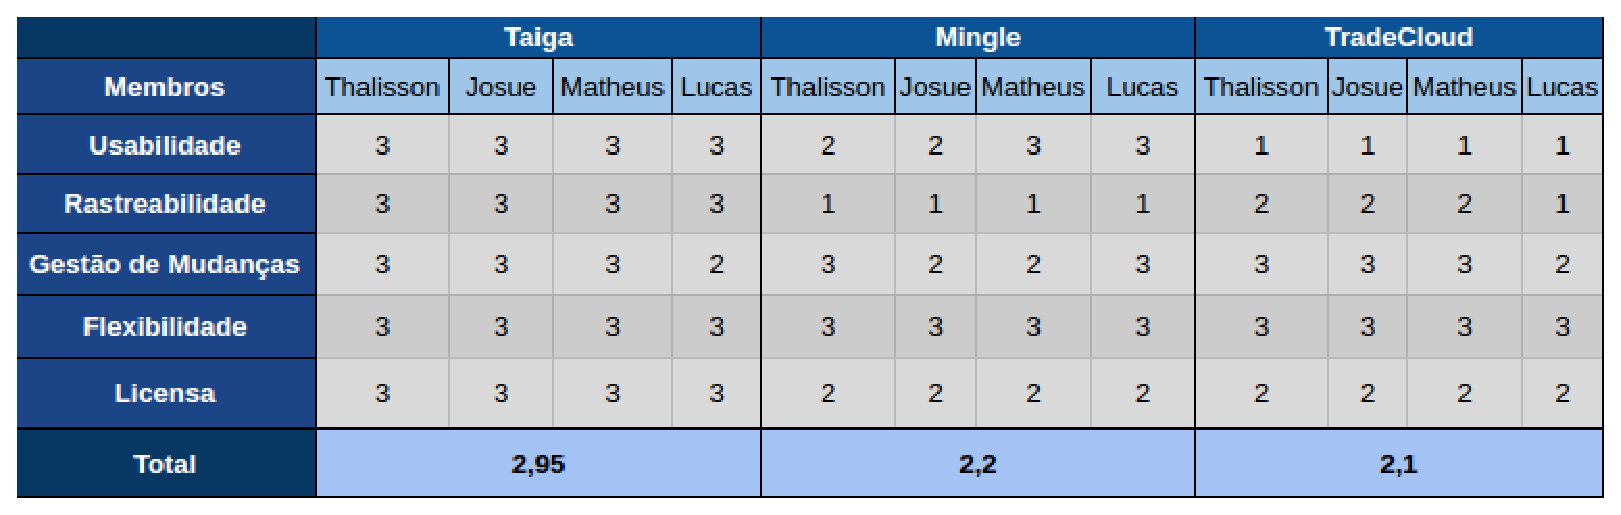
\includegraphics[keepaspectratio=true,scale=0.6]{figuras/votos.eps}
			\caption{Pontuação das Ferramentas}
			\label{fig15}
		  \end{figure}

\chapter{Planejamento do Projeto}
	\section{Cronograma}

	\begin{figure}[!h]
		 \centering
		 \includegraphics[keepaspectratio=true,scale=0.49]{figuras/cronograma.eps}
		 \caption{Cronograma}
		 \label{fig15}
	\end{figure}

\chapter{Considerações Finais}
Analisando cuidadosamente o contexto do cliente, foram detectadas dificuldades em algumas áreas, principalmente
na geração de conteúdo e gerenciamento das ferramentas de marketing e propaganda. Também ficou clara a disponibilidade
 do cliente de participar ativamente do processo, o que facilita a realização de reuniões mais frequentes.

Após constatar estes fatos, o grupo comparou diferentes metodologias para gestão de projetos e classificou a abordagem
 ágil, por meio do framework SAFe, mais adequada para a obtenção dos resultados esperados. Os processos descritos neste
 relatório permitem um desenvolvimento maduro, flexível, que permite a adaptação a mudanças e é consistente para a solução
  satisfatória dos problemas do cliente.

Por fim, este relatório abordou as informações, o planejamento e a base para o desenvolvimento do projeto como um
 todo, detalhando os resultados que o grupo pretende alcançar ao fim do projeto. Ele também permite a consulta para
  sanar  eventuais dúvidas que surjam ao longo do trabalho.
